\documentclass[../main.tex]{subfiles}

\begin{document}

\subsection{Parametric representations of lines}

\begin{example}
	Suppose that $L_1$ and $L_2$ are lines in the plane, that the
	x-intercepts of $L_1$ and $L_2$ are 5 and -1, respectively, and that the
	respective y-intercepts are 5 and 1. Find the point of intersection
	of $L_1$ and $L_2$.
\end{example}

\begin{solution}
	Pick two points on $L_1$,
	i.e. $(5, 0)$ and $(0, 5)$. Let $\vect{a}=\langle 5,\ 0\rangle$ and $\vect{b}=\langle 0,\ 5\rangle$.
	Now, $L_1$ can be represented by the following:

	\begin{equation*}
		\begin{split}
			L_1 & =  \{ (\vect{a} - \vect{b})t + \vect{b} \mid t \in \mathbb{R} \}                                \\
			    & =      \left. \left\{ \begin{bmatrix} 5t\\-5t+5 \end{bmatrix} \right| t \in \mathbb{R} \right\}
		\end{split}
	\end{equation*}

	The $(\vect{a} - \vect{b})t$ represents $L_1$ parameterized through the origin,
	so we apply a translation of $\vect{a}$ or $\vect{b}$. Similarly,
	let $\vect{c}= \langle -1, 0 \rangle$ and $\vect{d}= \langle 0, 1 \rangle$.

	\begin{equation*}
		\begin{split}
			L_2 & =  \{ (\vect{c} - \vect{d})s + \vect{d} \mid s \in \mathbb{R} \}                                 \\
			    & =      \left. \left\{ \begin{bmatrix} -s \\ -s+1 \end{bmatrix} \right| s \in \mathbb{R} \right\}
		\end{split}
	\end{equation*}

	The point of intersection is where $L_{1_x}=L_{2_x}$ and $L_{1_y}=L_{2_y}$,
	allowing us to define a system of equations.

	\begin{align*}
		5t= & -s & -5t+5=-s+1 \\
	\end{align*}

	\begin{align*}
		s= & -2     \\
		x= & -s=2   \\
		y= & -s+1=3
	\end{align*}

	The point of intersection is (2, 3). \qedsymbol
\end{solution}

\subsection{Linear dependence}

\begin{definition}[Linear combination]
	Let $V=\{ \vect{v_1}, \vect{v_2}, \ldots , \vect{v_k} \}$ where $\vect{v_i} \in \mathbb{R}^n$.
	A \textit{linear combination} of $V$ is defined to be
	$c_1\vect{v_1} + c_2\vect{v_2} + \dots + c_k\vect{v_k}$ where $c_i \in \mathbb{R}$.
\end{definition}

\begin{definition}[Linearly dependent]
	Let $V=\{ \vect{v_1}, \vect{v_2}, \ldots , \vect{v_k} \}$ where $\vect{v_i} \in \mathbb{R}^n$.
	$V$ is \textit{linearly dependent} if and only if
	$c_1\vect{v_1} + c_2\vect{v_2} + \dots + c_k\vect{v_k} = \vect{0}$
	where $c_i \in \mathbb{R}$ and there exists at least one $c_i$
	such that $c_i \neq 0$. In other words, $V$ is \textit{linearly independent}
	if and only if $c_1,c_2,\ldots ,c_k=0$ is the only solution.
\end{definition}

\begin{definition}[Span]
	Given a set $S$ of vectors, the \textit{span} of S,
	denoted $\operatorname{span}(S)$, is the set of all linear combinations of $S$.
\end{definition}

\begin{example}
	Let $S=\left\{
		\begin{bmatrix} 1 \\ -1 \\ 2 \end{bmatrix},
		\begin{bmatrix} 2 \\ 1 \\ 3 \end{bmatrix},
		\begin{bmatrix} -1 \\ 0 \\ 2 \end{bmatrix}
		\right\}$. Is $S$ linearly dependent?
\end{example}

\begin{solution}
	$$\begin{bmatrix} 1 \\ -1 \\ 2 \end{bmatrix}c_1
		+ \begin{bmatrix} 2 \\ 1 \\ 3 \end{bmatrix}c_2
		+ \begin{bmatrix} -1 \\ 0 \\ 2 \end{bmatrix}c_3 = 0$$

	\begin{equation*}
		\begin{split}
			c_1+2c_2-c_3   & =    \ 0     \\
			-c_1+c_2       & =        \ 0 \\
			2c_1+3c_2+2c_3 & =  \ 0
		\end{split}
	\end{equation*}

	Solving this system, we find that the only solution is
	$c_1=c_2=c_3=0$. Thus, $S$ is linearly independent. \qedsymbol
\end{solution}

We can go further by saying that the span of $S$ is $\mathbb{R}^3$. This
can be proven by setting the linear combination of $S$ to an
arbitrary 3-dimensional vector and isolating for the scalars $c_1$, $c_2$, and $c_3$,
which tells us that any given vector in $\mathbb{R}^3$ can be represented
in a specific linear combination of $S$. This can be thought of intuitively as well:
if $S$ is linearly independent, each vector of $S$ introduces
new directionality; there is no vector in $S$ that can be defined as a linear
combination of the other vectors.

\subsection{Linear subspaces}

\begin{definition}[Linear subspace]
	A set of vectors $V \subseteq \mathbb{R}^n$ is defined to be a linear/vector \textit{subspace}
	of $\mathbb{R}^n$ if and only if it contains $\vect{0}$,
	it is closed under scalar multiplication, and it is closed under addition:
	\begin{align*}
		\vect{0} \in                                                       & V \\
		\forall\ c \in \mathbb{R},\ c\vect{v} \in                          & V \\
		\forall\ \vect{v_1}, \vect{v_2} \in V, \vect{v_1} + \vect{v_2} \in & V
	\end{align*}
\end{definition}

\begin{theorem}
	Let $V=\{ \vect{v_1}, \vect{v_2}, \ldots , \vect{v_n} \}$. It holds true that
	$\operatorname{span}(V)$ is a subspace of $\mathbb{R}^n$.
\end{theorem}

\begin{proof}
	If $\operatorname{span}(V)$ is a valid linear subspace, it must contain the zero vector,
	it must be closed under scalar multiplication, and it must be closed
	under addition.

	By definition, the span of $V$ is the set of all linear combinations of $V$:
	\begin{equation*}
		\operatorname{span}(V)=\{ c_1\vect{v_1} + c_2\vect{v_2} + \dots + c_n\vect{v_n}\ \forall\ c_i \in \mathbb{R} \}
	\end{equation*}

	1. Inclusion of zero vector:
	\begin{center}
		Let $c_1, c_2, \ldots , c_n=0$.
		$$\implies c_1\vect{v_1} + c_2\vect{v_2} + \dots + c_n\vect{v_n}=\vect{0}$$
		$$\implies \vect{0} \in \operatorname{span}(V)$$
	\end{center}

	2. Closure under scalar multiplication:
	\begin{center}
		Let $\vect{a} \in \operatorname{span}(V)$.
		$$\iff c_1\vect{v_1} + c_2\vect{v_2} + \dots + c_n\vect{v_n}=\vect{a}$$
		$$d(c_1\vect{v_1} + c_2\vect{v_2} + \dots + c_n\vect{v_n})=d\vect{a}\ \textnormal{where}\ d \in \mathbb{R}$$
		$$\implies dc_1\vect{v_1} + dc_2\vect{v_2} + \dots + dc_n\vect{v_n}=d\vect{a}$$
	\end{center}

	$dc_i$ is just a scalar, meaning $d\vect{a}$ is another
	linear combination of $V$:
	$$d\vect{a} \in \operatorname{span}(V)$$

	3. Closure under addition:
	\begin{align*}
		\intertext{Let $\vect{a}, \vect{b} \in \operatorname{span}(V)$.}
		c_1\vect{v_1} + c_2\vect{v_2} + \dots + c_n\vect{v_n}                   & = \vect{a}            \\
		d_1\vect{v_1} + d_2\vect{v_2} + \dots + d_n\vect{v_n}                   & = \vect{b}            \\
		(c_1+d_1)\vect{v_1} + (c_2+d_2)\vect{v_2} + \dots + (c_n+d_n)\vect{v_n} & = \vect{a} + \vect{b}
	\end{align*}

	Again, $(c_i+d_i)$ is just a scalar, meaning $\vect{a}+\vect{b}$ is another linear combination of $V$:
	$$\vect{a}+\vect{b} \in \operatorname{span}(V)$$
\end{proof}

\begin{definition}[Basis]
	Let $S = \{ \vect{v_1}, \vect{v_2}, \ldots , \vect{v_n} \}$ be linearly independent.
	It follows that S is a \textit{basis} for the subspace $V = \operatorname{span}(S)$.
\end{definition}

\begin{lemma}
	Any vector in a subspace $V$ is the result of a unique linear combination
	of some basis for $V$.
\end{lemma}

\begin{proof}
	Let $S = \{ \vect{v_1}, \vect{v_2}, \ldots , \vect{v_n} \}$
	be a basis for the subspace $V$. Suppose $\vect{a} \in V$.
	\begin{align*}
		\vect{a} & = c_1\vect{v_1}+c_2\vect{v_2} + \dots + c_n\vect{v_n}\ \textnormal{where}\ c_i \in \mathbb{R} \\
		\intertext{Assume that $\vect{a}$ can be represented by another linear combination
			of $S$.}
		\vect{a} & = d_1\vect{v_1} + d_2\vect{v_2} + \dots + d_n\vect{v_n}\ \textnormal{for some}\ d_j \neq c_j  \\
		\vect{0} & = (c_1-d_1)\vect{v_1} + (c_2-d_2)\vect{v_2} + \dots + (c_n-d_n)\vect{v_n}
	\end{align*}

	S is linearly independent so the scalar $(c_i-d_i)$ must be zero for $1 \leq i \leq n$.
	This implies that $c_i=d_i$ which contradicts the statement that some $d_j \neq c_j$.
	This further implies that $\vect{a}$ cannot be represented by more than
	one linear combination of $S$.
\end{proof}

\subsection{Dot product}

\begin{definition}
	The \textit{dot product} of two vectors $\vect{a}, \vect{b} \in \mathbb{R}^n$, denoted
	$\vect{a} \cdot \vect{b}$, is defined to be
	${\vect{a} \cdot \vect{b} = \vect{a_1}\vect{b_1} + \vect{a_2}\vect{b_2} + \dots + \vect{a_n}\vect{b_n}}$.
\end{definition}

\begin{lemma}
	$\vect{a} \cdot \vect{a} = \|\vect{a}\| ^2$.
\end{lemma}

\begin{proof}
	Let $\vect{a} \in \mathbb{R}^n$.
	\begin{align*}
		\|\vect{a}\|   & = \sqrt{a_1^2+a_2^2+\dots + a_n^2} \\
		\|\vect{a}\|^2 & = |a_1^2+a_2^2+\dots + a_n^2|      \\
		               & = a_1^2+a_2^2+\dots + a_n^2        \\
		               & = \vect{a}\cdot\vect{a}
	\end{align*}
\end{proof}

\subsubsection{Properties}

Dot products are commutative ($\vect{a} \cdot \vect{b} = \vect{b} \cdot \vect{a}$),
distributive ($\vect{a} \cdot (\vect{b} + \vect{c}) = \vect{a} \cdot \vect{b} + \vect{a} \cdot \vect{c}$),
and associative with scalars ($c(\vect{a} \cdot \vect{b}) = (c\vect{a}) \cdot \vect{b} = \vect{a} \cdot (c\vect{b})$).
These properties can be easily proven with the definition of the dot product.

\subsubsection{Geometric representation}

The dot product of two vectors can also
be represented in relation to the angle between them, $\theta$, by
the following: $\vect{a} \cdot \vect{b} = \|\vect{a}\| \|\vect{b}\| \cos (\theta)$.

\begin{figure}[H]
	\centering
	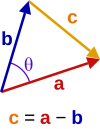
\includegraphics[width=70px]{Dot_product_cosine_rule.svg.png}
	\caption{The angle $\theta$ in the triangle constructed
		by $\vect{a}$, $\vect{b}$, and $\vect{a} - \vect{b}$}
\end{figure}

\begin{proof}
	Let $\vect{a}, \vect{b} \in \mathbb{R}^n$ such that $\vect{a}, \vect{b} \neq 0$. Using the Law of Cosines,
	\begin{align*}
		\|\vect{a}-\vect{b}\|^2                                    & = \|\vect{a}\|^2 + \|\vect{b}\|^2 - 2\|\vect{a}\| \|\vect{b}\| \cos (\theta) \\
		\|\vect{a}\|^2 - 2(\vect{a}\cdot\vect{b}) + \|\vect{b}\|^2 & = \|\vect{a}\|^2+\|\vect{b}\|^2-2\|\vect{a}\|\|\vect{b}\|\cos (\theta)       \\
		-2(\vect{a}\cdot\vect{b})                                  & =-2\|\vect{a}\|\|\vect{b}\|\cos (\theta)                                     \\
		\vect{a}\cdot\vect{b}                                      & =\|\vect{a}\|\|\vect{b}\|\cos (\theta)                                       \\
	\end{align*}
\end{proof}

\subsubsection{Interpretation}

The geometric representation makes it easy to recognize that
$\vect{a}\cdot\vect{b}$ is maximized when $\theta=0\degree$, which is
when $\vect{a}$ and $\vect{b}$ are collinear in the same direction.
On the other hand, $\vect{a}\cdot\vect{b}$ is minimized when $\theta=180\degree$,
which is when $\vect{a}$ and $\vect{b}$ are collinear in opposite directions.
When $\vect{a}$ and $\vect{b}$ are perpendicular to each other (i.e. $\theta=90\degree$),
$\vect{a}\cdot\vect{b}=0$. This means that we can interpret the dot product as a measure
of collinearity.

\begin{definition}[Orthogonal]
	Vectors $\vect{a}, \vect{b} \in \mathbb{R}^n$ are \textit{orthogonal} to each other if and only if $\vect{a}\cdot\vect{b}=0$.
\end{definition}

\subsubsection{Cauchy-Schwarz Inequality}

\begin{lemma}
	For some scalar $c \geq 0$ and some vector $\vect{a}$, $c\|\vect{a}\|=\|c\vect{a}\|$.
\end{lemma}

\begin{proof}
	Let $c \geq 0, c \in \mathbb{R}$. Let $\vect{a} \in \mathbb{R}^n$.
	\begin{align*}
		c\|\vect{a}\| & = c\sqrt{a_1^2+a_2^2+\dots +a_n^2}         \\
		              & = \sqrt{c^2(a_1^2+a_2^2+\dots +a_n^2)}     \\
		              & = \sqrt{(ca_1)^2+(ca_2)^2+\dots +(ca_n)^2} \\
		              & = \|c\vect{a}\|
	\end{align*}
\end{proof}

\begin{theorem}[Cauchy-Schwarz inequality] \label{cauchy_schwarz}
	If $\vect{x}, \vect{y} \in \mathbb{R}^n$, then
	$\|\vect{x}\|\|\vect{y}\| \geq |\vect{x}\cdot\vect{y}|$. Furthermore,
	$\|\vect{x}\|\|\vect{y}\|=|\vect{x}\cdot\vect{y}|$ if and only if $\vect{y}=c\vect{x}$
	for some $c \in \mathbb{R}$.
\end{theorem}

\begin{proof}
	Let $\vect{x}, \vect{y} \in \mathbb{R}^n$ be nonzero.
	Let $p(t)=\|t\vect{y}-\vect{x}\|^2$. Note that $p(t) \geq 0$ for all $t \in \mathbb{R}$.
	\begin{align*}
		p(t)                         & =  (t\vect{y}-\vect{x})\cdot(t\vect{y}-\vect{x})                  \\
		                             & =      t^2\|\vect{y}\|^2-2t(\vect{x}\cdot\vect{y})+\|\vect{x}\|^2
		\intertext{Let $a=\|\vect{y}\|^2$. Let $b=2(\vect{x}\cdot\vect{y})$. Let $c=\|\vect{x}\|^2$.
			Note that $a \neq 0$ because $\vect{y} \neq \vect{0}$.}
		p(t)                         & =at^2-bt+c \geq 0                                                 \\
		p\left(\frac{b}{2a}\right)   & =a\left(\frac{b}{2a}\right)^2-b\left(\frac{b}{2a}\right)+c        \\
		                             & = \frac{b^2}{4a}-\frac{b^2}{2a}+c                                 \\
		                             & = -\frac{b^2}{4a}+c \geq 0                                        \\
		\implies c                   & \geq \frac{b^2}{4a}
		\intertext{Substituting back $a$, $b$, and $c$:}
		\|\vect{x}\|^2               & \geq \frac{4(\vect{x}\cdot\vect{y})^2}{4\|\vect{y}\|^2}           \\
		\|\vect{x}\|^2\|\vect{y}\|^2 & \geq (\vect{x}\cdot\vect{y})^2                                    \\
		\|\vect{x}\|\|\vect{y}\|     & \geq |\vect{x}\cdot\vect{y}|
	\end{align*}

	Consider the case of the equality:
	\begin{align*}
		\|\vect{x}\|\|\vect{y}\| & = |\vect{x}\cdot\vect{y}|                 \\
		\|\vect{x}\|\|\vect{y}\| & = |\|\vect{x}\|\|\vect{y}\|\cos (\theta)|
	\end{align*}
	This can be true if and only if $\theta=0\degree$ or $\theta=180\degree$,
	meaning $\vect{x}$ and $\vect{y}$ must be collinear with each other.

	While we initially assumed that $\vect{x}$ and $\vect{y}$ were nonzero,
	it is easy to see that the inequality still holds when $\vect{x}=\vect{0}$ or $\vect{y}=\vect{0}$.
\end{proof}

\begin{theorem}[Triangle inequality]
	If $\vect{x}, \vect{y} \in \mathbb{R}^n$, then
	$\|\vect{x}+\vect{y}\| \leq \|\vect{x}\|+\|\vect{y}\|$. This inequality
	becomes an equality if and only if $\vect{y}=c\vect{x}$ for some
	$c \in \mathbb{R}$ such that $c\geq0$. In other words, the sum of
	the lengths of two sides of a triangle is always greater than the
	length of its third side.
\end{theorem}

\begin{figure}[H]
	\centering
	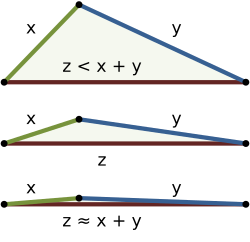
\includegraphics[width=200px]{TriangleInequality.svg.png}
	\caption{As two sides of a triangle get closer to being collinear,
		the sum of their lengths gets closer to the length of the third side.}
\end{figure}

\begin{proof}
	Let $\vect{x}, \vect{y} \in \mathbb{R}^n$.
	By the Cauchy-Schwarz inequality (Theorem \ref{cauchy_schwarz}),
	$$\|\vect{x}\|\|\vect{y}\|\geq |\vect{x}\cdot\vect{y}|\geq\vect{x}\cdot\vect{y}$$
	Note that $|\vect{x}\cdot\vect{y}|=\vect{x}\cdot\vect{y}$ if and only if
	$\vect{x}\cdot\vect{y}\geq0$. Else, $|\vect{x}\cdot\vect{y}|>\vect{x}\cdot\vect{y}$.
	Additionally, $|\vect{x}\cdot\vect{y}|=\|\vect{x}\|\|\vect{y}\|$ if and only if
	$\vect{y}=c\vect{x}$ for some $c \in \mathbb{R}$, as stated in the Cauchy-Schwarz inequality.
	So, if $c\geq0$ and $\vect{y}=c\vect{x}$, then
	$\vect{x}\cdot\vect{y}=|\vect{x}\cdot\vect{y}|=\|\vect{x}\|\|\vect{y}\|$.

	Now, consider the following:
	$$\|\vect{x} + \vect{y}\|^2  = \|\vect{x}\|^2+2(\vect{x}\cdot\vect{y})+\|\vect{y}\|^2 $$
	Since $\|\vect{x}\|\|\vect{y}\|\geq\vect{x}\cdot\vect{y}$,
	we can create the inequality $\|\vect{x}+\vect{y}\|^2\leq\|\vect{x}\|^2+2\|\vect{x}\|\|\vect{y}\|+\|\vect{y}\|^2$.
	Note that this inequality becomes an equality if and only if $\vect{y}=c\vect{x}$.
	\begin{align*}
		\|\vect{x}+\vect{y}\|^2   & \leq\ |\vect{x}\|^2+2\|\vect{x}\|\|\vect{y}\|+\|\vect{y}\|^2 \\
		\|\vect{x} + \vect{y}\|^2 & \leq (\|\vect{x}\|+\|\vect{y}\|)^2                           \\
		\|\vect{x} + \vect{y}\|   & \leq \|\vect{x}\|+\|\vect{y}\|
	\end{align*}
\end{proof}

\subsection{Cross product}

\begin{definition}
	The \textit{cross product} of two vectors $\vect{a}, \vect{b} \in \mathbb{R}^3$,
	denoted $\vect{a}\times\vect{b}$, is defined to be
	\begin{align*}
		\vect{a}\times\vect{b} & = \begin{bmatrix}a_1\\a_2\\a_3\end{bmatrix}\times\begin{bmatrix}b_1\\b_2\\b_3\end{bmatrix} \\
		                       & = \begin{bmatrix}a_2b_3-a_3b_2\\a_3b_1-a_1b_3\\a_1b_2-a_2b_1\end{bmatrix}
	\end{align*}
\end{definition}

\begin{remark}
	A way to easily remember how to calculate the cross product is by writing
	it as a determinant (covered in Section ??):
	$$\vect{a}\times\vect{b}=\begin{vmatrix}
			\uvec{\imath} & \uvec{\jmath} & \uvec{k} \\
			a_1           & a_2           & a_3      \\
			b_1           & b_2           & b_3
		\end{vmatrix}$$
\end{remark}
\end{document}
